\documentclass{minimal}
\usepackage{tikz}
\usetikzlibrary{calc,trees,positioning,arrows,chains,shapes.geometric,%
    decorations.pathreplacing,decorations.pathmorphing,shapes,%
    matrix,shapes.symbols}

\tikzset{
>=stealth',
  punktchain/.style={
    rectangle, 
    rounded corners, 
    % fill=black!10,
    draw=black, very thick,
    text width=10em, 
    minimum height=3em, 
    text centered, 
    on chain},
  line/.style={draw, thick, <-},
  element/.style={
    tape,
    top color=white,
    bottom color=blue!50!black!60!,
    minimum width=8em,
    draw=blue!40!black!90, very thick,
    text width=10em, 
    minimum height=3.5em, 
    text centered, 
    on chain},
  every join/.style={->, thick,shorten >=1pt},
  decoration={brace},
  tuborg/.style={decorate},
  tubnode/.style={midway, right=2pt},
}

\def\position{\mathrm{x}}
\def\speed{\mathrm{v}}
\def\acceleration{\mathrm{\gamma}}
\def\forcet{\mathrm{F_t}}
\def\forcer{\mathrm{F_r}}
\def\masse{\mathrm{m}}

%%%%%%%%%%%%%%%%%%%
\def\ProfileProject{\mathrm{Ps}}
%%%%%%%%%%%%%%%%

\begin{document}
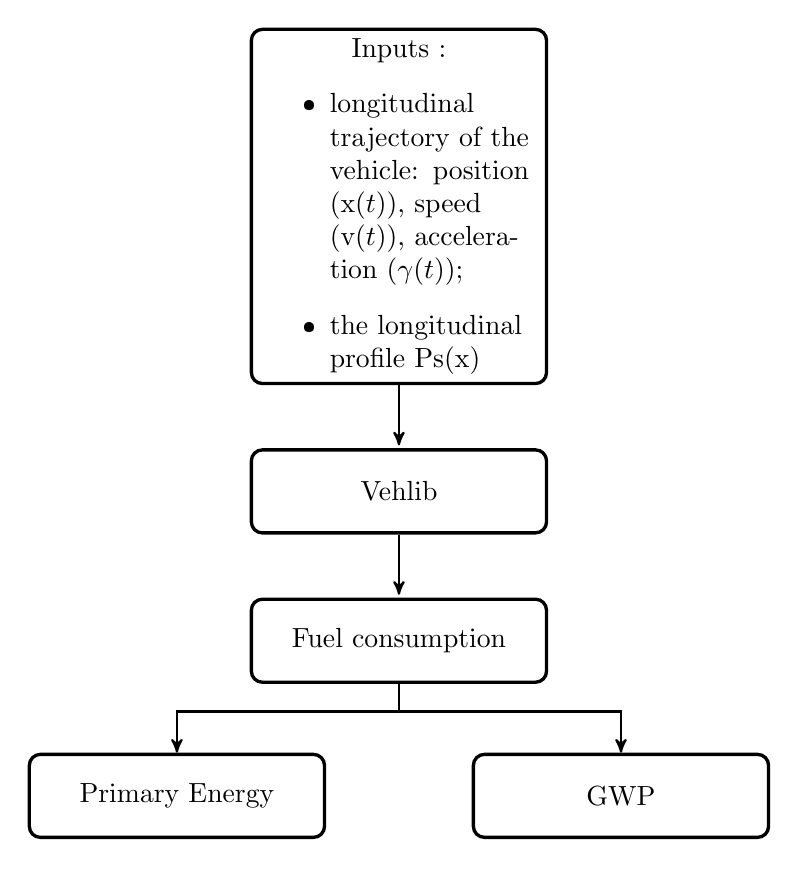
\begin{tikzpicture}
  [node distance=.8cm,
  start chain=going below,]
	\node[punktchain, join] (intro) {Inputs : \begin{itemize}
		\item longitudinal trajectory of the vehicle: position ($\position(t)$), speed ($\speed(t)$), acceleration ($\gamma(t)$);
		\item  the longitudinal profile $\ProfileProject(\position)$ 
			\end{itemize} 
			};
     \node[punktchain, join] (probf)      {Vehlib};
     \node[punktchain, join] (investeringer)      {Fuel consumption};
     %\node[punktchain, join] (perfekt) {Det perfekte kapitalmarked};
     %\node[punktchain, join, ] (emperi) {Emperi};
      \node (asym) [on chain, minimum height=3.5em]  {};
      \begin{scope}[start branch=venstre,
        %We need to redefine the join-style to have the -> turn out right
        every join/.style={->, thick, shorten <=1pt}, ]
        \node[punktchain, on chain=going left]
            (risiko) {Primary Energy};
      \end{scope}
      \begin{scope}[start branch=hoejre,]
      \node (finans) [punktchain, on chain=going right] {GWP};
	      \draw[|-,-|,->, thick,] (investeringer.south) |-+(0,-1em)-| (risiko.north);
 \draw[|-,-|,->, thick,] (investeringer.south) |-+(0,-1em)-| (finans.north);

    \end{scope}
 % \node[punktchain, join,] (disk) {Det imperfekte finansielle marked};
 % \node[punktchain, join,] (makro) {Investeringsmæssige konsekvenser};
 % \node[punktchain, join] (konk) {Konklusion};
  % Now that we have finished the main figure let us add some "after-drawings"
  %% First, let us connect (finans) with (disk). We want it to have
  %% square corners.
%  \draw[|-,-|,->, thick,] (finans.south) |-+(0,-1em)-| (disk.north);
  % Now, let us add some braches. 
  %% No. 1
  %\draw[tuborg] let
   % \p1=(risiko.west), \p2=(finans.east) in
   % ($(\x1,\y1+2.5em)$) -- ($(\x2,\y2+2.5em)$) node[above, midway]  {Teori};
  %% No. 2
  %\draw[tuborg, decoration={brace}] let \p1=(disk.north), \p2=(makro.south) in
   % ($(2, \y1)$) -- ($(2, \y2)$) node[tubnode] {Analyse};
  %% No. 3
  %\draw[tuborg, decoration={brace}] let \p1=(perfekt.north), \p2=(emperi.south) in
   % ($(2, \y1)$) -- ($(2, \y2)$) node[tubnode] {Problemfelt};
  \end{tikzpicture}
  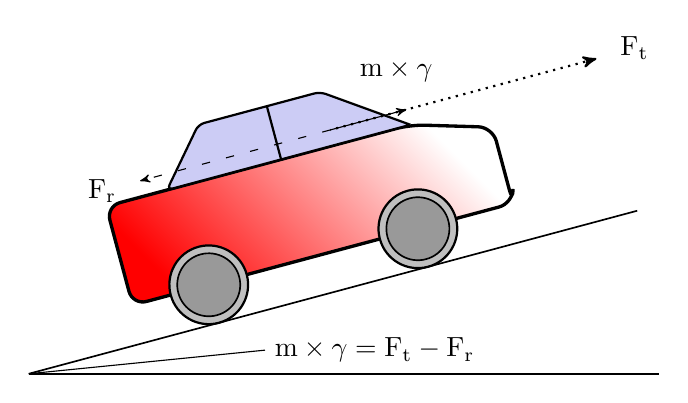
\begin{tikzpicture}
	   \begin{scope}[rotate=15]
	  \begin{scope}[xscale=-1]
    \shade[top color=red, bottom color=white, shading angle={135}]
        [draw=black,fill=red!20,rounded corners=1.2ex,very thick] (1.5,.5) -- ++(0,1) -- ++(1,0.3) --  ++(3,0) -- ++(1,0) -- ++(0,-1.3) -- (1.5,.5) -- cycle;
    \draw[very thick, rounded corners=0.5ex,fill=black!20!blue!20!white,thick]  (2.5,1.8) -- ++(1,0.7) -- ++(1.6,0) -- ++(0.6,-0.7) -- (2.5,1.8);
    \draw[thick]  (4.2,1.8) -- (4.2,2.5);
    \draw[draw=black,fill=gray!50,thick] (2.75,.5) circle (.5);
    \draw[draw=black,fill=gray!50,thick] (5.5,.5) circle (.5);
    \draw[draw=black,fill=gray!80,semithick] (2.75,.5) circle (.4);
    \draw[draw=black,fill=gray!80,semithick] (5.5,.5) circle (.4);
		  \draw[<-,thick, dotted] (0,2) -- (3.5,2);   \draw (-0.5,2) node {$\forcet$};
		  \draw[->] (3.5,2) -- (2.5,2);   \draw (2.5,2.5) node {$\masse\times\acceleration$};
		  \draw[->,loosely dashed] (3.5,2) -- (6,2);   \draw (6.5,2) node {$\forcer$};
		  \draw[semithick] (0,0) -- (8,0);
		  \coordinate (debut) at (8,0) ;

	   \end{scope}
		    \end{scope}
%    \draw[->,thick] (-3.5,0) -- (0,3);\draw (0,3.5) node {$\ProfileProject$};
    \draw[-,thick] (debut) -- ++(8,0);
	  \draw (debut)-- ++(3,0.3)  node[right] {$\masse\times\acceleration = \forcet - \forcer  $};

%     \draw[->,thick] (debut) -- ++(0,0);


\end{tikzpicture}

  \end{document}
%%% Local Variables: 
%%% mode: latex
%%% TeX-master: t
%%% End: 

